\usetikzlibrary{arrows.meta,calc}
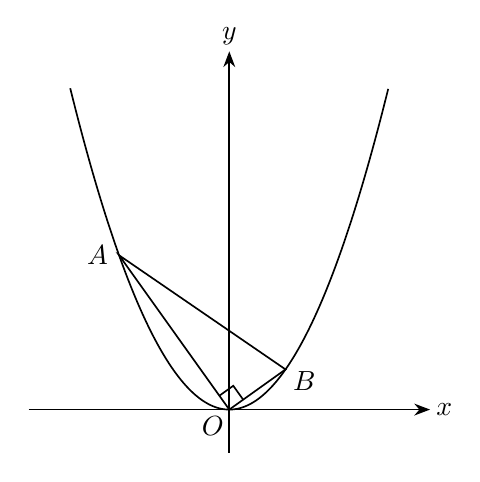
\begin{tikzpicture}[x=1cm,y=1cm,line width=.6pt,>=Stealth,font=\normalsize]
\coordinate (O) at (0,0);
\coordinate (A) at (-1.4,1.96);
\coordinate (B) at (0.7142857,0.5102041);
\coordinate (U) at (-0.1260124,0.1764174);
\coordinate (V) at (0.1764174,0.1260124);
\coordinate (W) at (0.0504050,0.3024299);
\draw[->] (-2.55,0)--(2.55,0);
\draw[->] (0,-0.55)--(0,4.55);
\draw[domain=-2.02:2.02,samples=161] plot (\x,{\x*\x});
\draw (A)--(O)--(B)--cycle;
\draw (U)--(W)--(V);
\node[anchor=north east,inner sep=0pt] at (-0.06,-0.08) {$O$};
\node[anchor=east,inner sep=0pt] at (-1.53,1.96) {$A$};
\node[anchor=west,inner sep=0pt] at (0.8,0.36) {$B$};
\node[anchor=west,inner sep=0pt] at (2.62,0) {$x$};
\node[anchor=south,inner sep=0pt] at (0,4.62) {$y$};
\end{tikzpicture}
